\documentclass{article}

\usepackage{graphicx}
\usepackage{tikz}
\usepackage{tikzsymbols}
\usetikzlibrary{calc,patterns,shapes.geometric}
\pagestyle{empty}
\usepackage[margin=0pt]{geometry}
\geometry{papersize={14in,12in}}

\def\centerarc[#1](#2)(#3:#4:#5){\draw[#1] ($(#2)+({#5*cos(#3)},{#5*sin(#3)})$) arc (#3:#4:#5);}

\begin{document}
	\begin{figure}
		\centering
		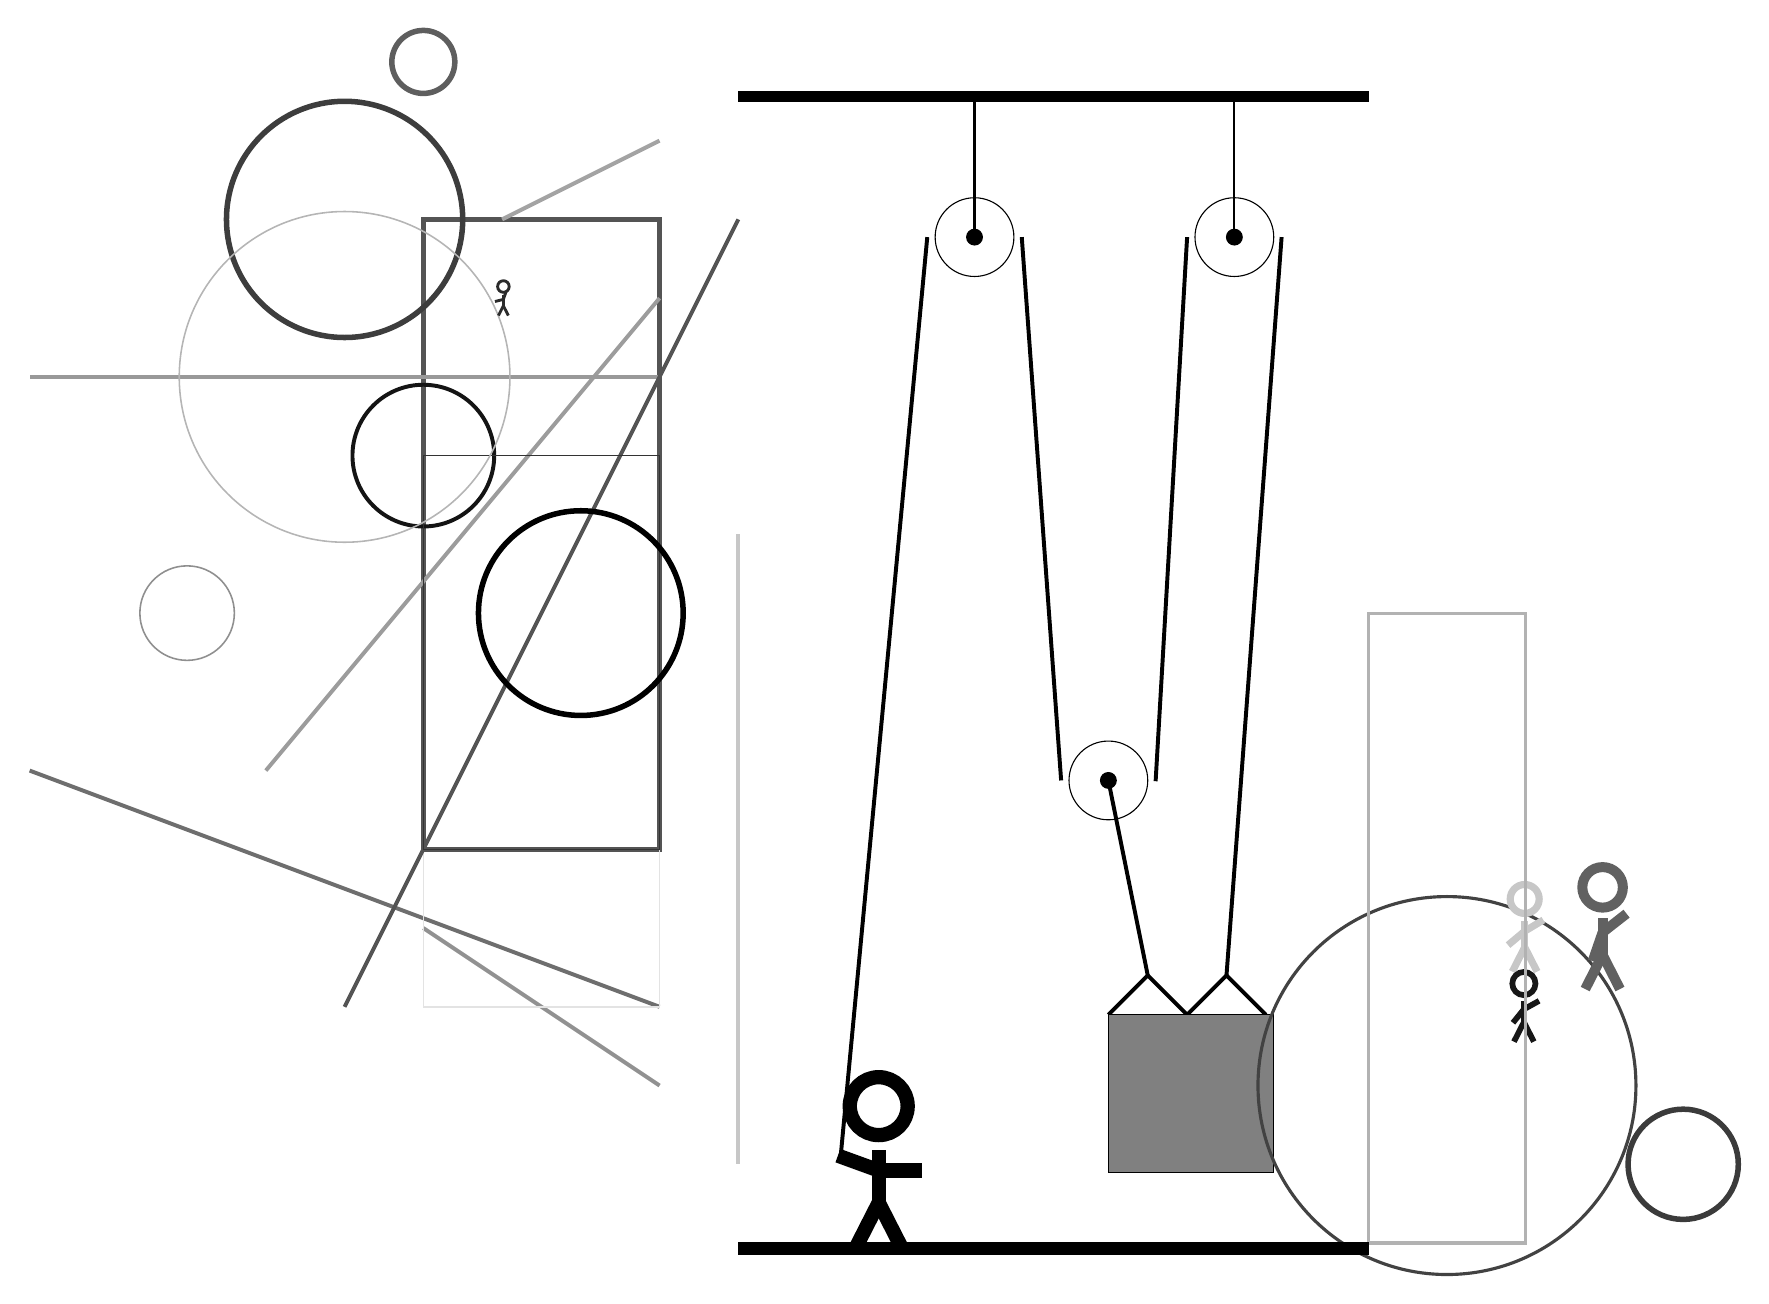
\begin{tikzpicture}
			%%%%% START %%%%%
			
			\draw[fill=black] (-2, 11.5) rectangle (6, 11.625);
			
			\draw (1, 9.775) circle (0.5);
			\draw[fill=black] (1, 9.775) circle (0.1);
			\draw[thick] (1, 9.775) -- (1, 11.5);
			
			\draw (4.3, 9.775) circle (0.5);
			\draw[fill=black] (4.3, 9.775) circle (0.1);
			\draw[thick] (4.3, 9.775) -- (4.3, 11.5);
			
			\draw (2.7, 2.875) circle (0.5);
			\draw[fill=black] (2.7, 2.875) circle (0.1);
			
			\draw[line width=0.5mm]  (2.7, -0.1) -- (3.2, 0.4) -- (3.7, -0.1) -- (4.2, 0.4) -- (4.7, -0.1);
			\draw[fill=black!50] (2.7, -0.1) rectangle (4.8, -2.1);
			
			\draw[line width=0.5mm](-0.7, -1.9) -- (0.4, 9.775);
			\centerarc[line width=0.5mm](1, 9.775)(0:180:0.6);
			\draw[line width=0.5mm](1.6, 9.775) -- (2.1, 2.875);
			\centerarc[line width=0.5mm](2.7, 2.875)(180:370:0.6);
			\draw[line width=0.5mm] (3.3, 2.865) -- (3.7, 9.775);
			\centerarc[line width=0.5mm](4.3, 9.775)(0:180:0.6);
			\draw[line width=0.5mm](4.2, 0.4) -- (4.9, 9.775);
			\draw[line width=0.5mm] (3.2, 0.4) -- (2.7, 2.875);
			
			\draw [line width=0.4mm, color=black!74](7, -1) circle (2.4);
			
			\draw[line width=0.5mm, color=black!22](-2, 6) -- (-2, -2);
			\draw [line width=0.2mm, color=black!44](-9, 5) circle (0.6);
			\draw[line width=0.6mm, color=black!67] (-3, 10) rectangle (-6, 2);
			\draw [line width=0.5mm, color=black!92](-6, 7) circle (0.9);
			\draw[line width=0.5mm, color=black!57](-3, 0) -- (-11, 3);
			\draw[line width=0.5mm, color=black!43](-3, -1) -- (-6, 1);
			
			\draw[line width=0.2mm, color=black!11] (-3, 0) rectangle (-6, 2);
			\draw[line width=0.5mm, color=black!36](-3, 11) -- (-5, 10);
			\draw[line width=0.5mm, color=black!39](-3, 9) -- (-8, 3);
			\node[line width=0.5mm, color=black!22] at (8, 1) {\Strichmaxerl[5][40][31]};
			\draw[line width=0.6mm, color=black!37] (-2, -3) rectangle (-2, -3);
			\draw[line width=0.5mm, color=black!40](-3, 8) -- (-11, 8);
			
			\draw[line width=0.5mm, color=black!67](-7, 0) -- (-2, 10);
			\draw[line width=0.2mm, color=black!80] (-3, 7) rectangle (-6, 2);
			\node[line width=0.3mm, color=black!62] at (9, 1) {\Strichmaxerl[7][71][38]};
			
			\node[line width=0.7mm, color=black!91] at (8, 0) {\Strichmaxerl[4][51][29]};
			
			\draw [line width=0.7mm, color=black!63](-6, 12) circle (0.4);
			\draw[line width=0.4mm, color=black!30] (6, 5) rectangle (8, -3);
			
			\draw [line width=0.7mm, color=black!77](10, -2) circle (0.7);
			\draw [line width=0.7mm, color=black!100](-4, 5) circle (1.3);
			
			\draw [line width=0.7mm, color=black!76](-7, 10) circle (1.5);
			\draw [line width=0.2mm, color=black!29](-7, 8) circle (2.1);
			\node[line width=0.6mm, color=black!83] at (-5, 9) {\Strichmaxerl[2][14][71]};
			
			\node at (-0.2, -2) {\Strichmaxerl[10][-20][0]};
			
			\draw[fill=black] (-2, -3) rectangle (6, -3.15);
			
			%%%%% END %%%%%
		\end{tikzpicture}
	\end{figure}	
\end{document}